% Q8：逐点复现原页的五个空心圆点阵，不据此添加题目未给的几何条件。
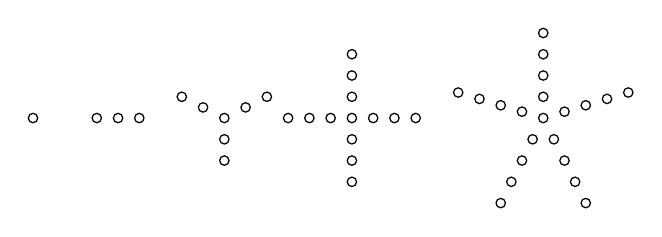
\begin{tikzpicture}[x=0.27cm,y=0.27cm,line width=0.45pt]
  \foreach \x/\y in {
    0/0,
    3/0,4/0,5/0,
    7/1,8/0.5,9/0,10/0.5,11/1,9/-1,9/-2,
    15/-3,15/-2,15/-1,15/0,15/1,15/2,15/3,
    12/0,13/0,14/0,16/0,17/0,18/0,
    24/4,24/3,24/2,24/1,
    20/1.2,21/0.9,22/0.6,23/0.3,24/0,25/0.3,26/0.6,27/0.9,28/1.2,
    23.5/-1,24.5/-1,23/-2,25/-2,22.5/-3,25.5/-3,22/-4,26/-4
  } {
    \draw[fill=white] (\x,\y) circle[radius=1.7pt];
  }
\end{tikzpicture}
